\subsection{RQ2:  Coverage with Rex}
\label{sec:rq3}
\iffalse
\begin{table}[tb]
\caption{Description of 12,181 regular expressions analyzed in Rex of Unicode encoding.}
\label{rex:unicode}
\begin{small}
\begin{tabular}{p{2cm}
>{\raggedleft\arraybackslash}p{0.6cm}
>{\raggedleft\arraybackslash}p{0.6cm}
>{\raggedleft\arraybackslash}p{0.6cm}
>{\raggedleft\arraybackslash}p{0.6cm}
>{\raggedleft\arraybackslash}p{0.6cm}
>{\raggedleft\arraybackslash}p{0.6cm}}
\hline
Attributes & mean & 25\% & 50\% & 75\% & 90\% & 99\%  \\  
\hline
Nodes& 157 & 13 & 31 & 89 & 429 & 952 \\  
Edges& 550 & 27 & 79 & 262 & 1,119 & 2,896 \\  
Edge pairs& 1,738 & 32 & 108 & 513 & 1,739 & 18,156 \\
%Unique inputs&  &     &     &   &   &   \\  
Regular exp. len. & 31  & 14 & 18 & 40 & 68 & 146 \\
%Input length avg. &  &  &  &  &  &  \\  
%Input length dev. &  &  &  &  &  &  \\
\hline
\end{tabular}

\vspace{3pt}
All deviations are rounded to 2 decimal places. All input length averages are rounded to nearest integer.
\end{small}
\end{table}


\begin{table}[tb]
\caption{Description of 12,184 regular expressions analyzed in Rex of ASCII encoding.}
\label{rex:ascii}
\begin{small}
\begin{tabular}{p{2cm}
>{\raggedleft\arraybackslash}p{0.6cm}
>{\raggedleft\arraybackslash}p{0.6cm}
>{\raggedleft\arraybackslash}p{0.6cm}
>{\raggedleft\arraybackslash}p{0.6cm}
>{\raggedleft\arraybackslash}p{0.6cm}
>{\raggedleft\arraybackslash}p{0.6cm}}
\hline
Attributes & mean & 25\% & 50\% & 75\% & 90\% & 99\%  \\  
\hline
Nodes& 157 & 13 & 31 & 89 & 429 & 952 \\  
Edges& 550 & 27 & 79 & 262 & 1,118 & 2,895 \\  
Edge pairs& 1,738 & 32 & 108 & 513 & 1,739 & 18,153 \\
%Unique inputs&  &     &     &   &   &   \\  
Regular exp. len. & 31  & 14 & 18 & 40 & 68 & 146 \\
%Input length avg. &  &  &  &  &  &  \\  
%Input length dev. &  &  &  &  &  &  \\
\hline
\end{tabular}

\vspace{3pt}
All deviations are rounded to 2 decimal places. All input length averages are rounded to nearest integer.
\end{small}
\end{table}
\fi

\begin{figure*}[t]
	\centering
	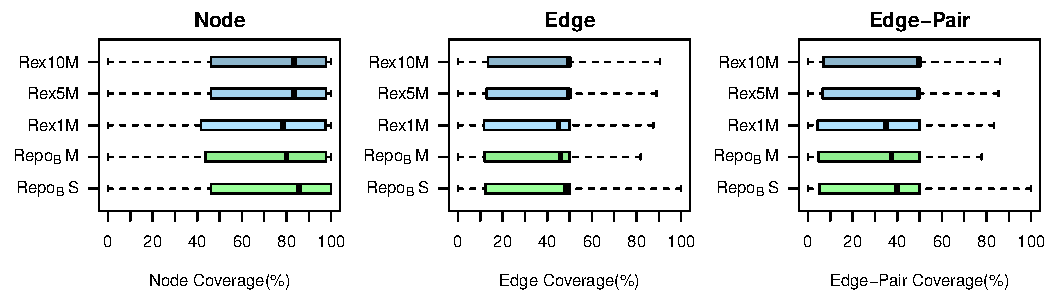
\includegraphics[width=\textwidth]{figures/rexCovASCII2Embed}
%	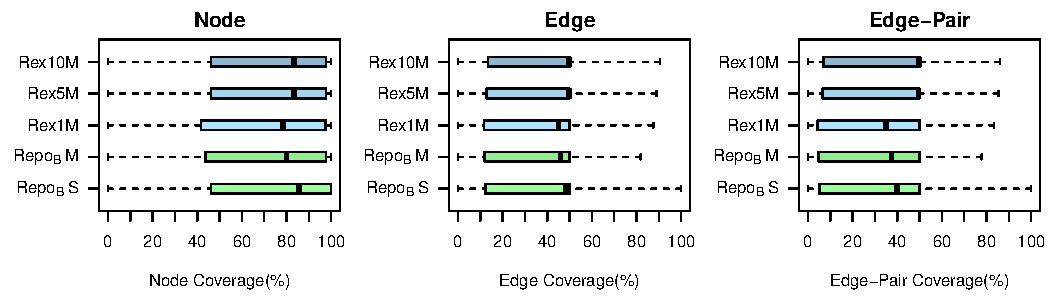
\includegraphics[width=\textwidth]{figures/rexCovASCII2}
	\vspace{-24pt}
%	\caption{Node, edge, edge-pair coverage of 7,886 regular expressions with Rex-generated ASCII inputs of successful matchings from Rex and with the number of successful inputs in GitHub projects}
	\caption{Node, edge, edge-pair coverage of 7,926 regular expressions with Rex-generated ASCII inputs ($Rex1M$, $Rex5M$, $Rex10M$) of 7,926 regular expressions in GitHub which are used in Rex ($Repo_{B}S$, $Repo_{B}M$).}
	\label{cov:ascii}    
%	\vspace{-3pt}
\end{figure*}

\iffalse
\begin{figure}[t]
	\centering
	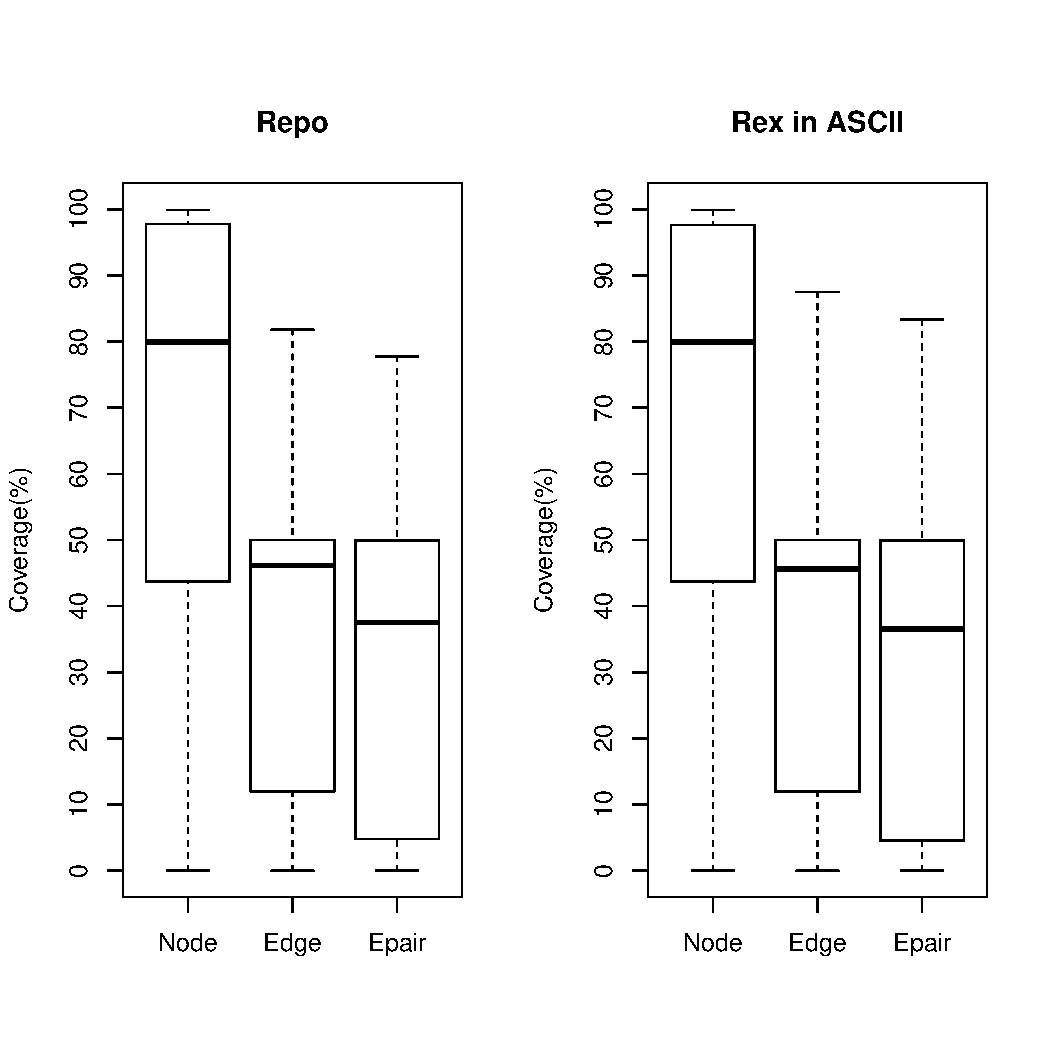
\includegraphics[width=0.5\textwidth]{figures/rexCovASCIIS1}
	\vspace{-6pt}
	\caption{Node, edge, edge-pair coverage of 7,886 regular expressions with Rex-generated ASCII inputs of successful matchings from Rex and with the number of successful inputs in GitHub projects}
	\label{cov:ascii}    
	\vspace{-6pt}
\end{figure}
\begin{figure}[t]
	\centering
	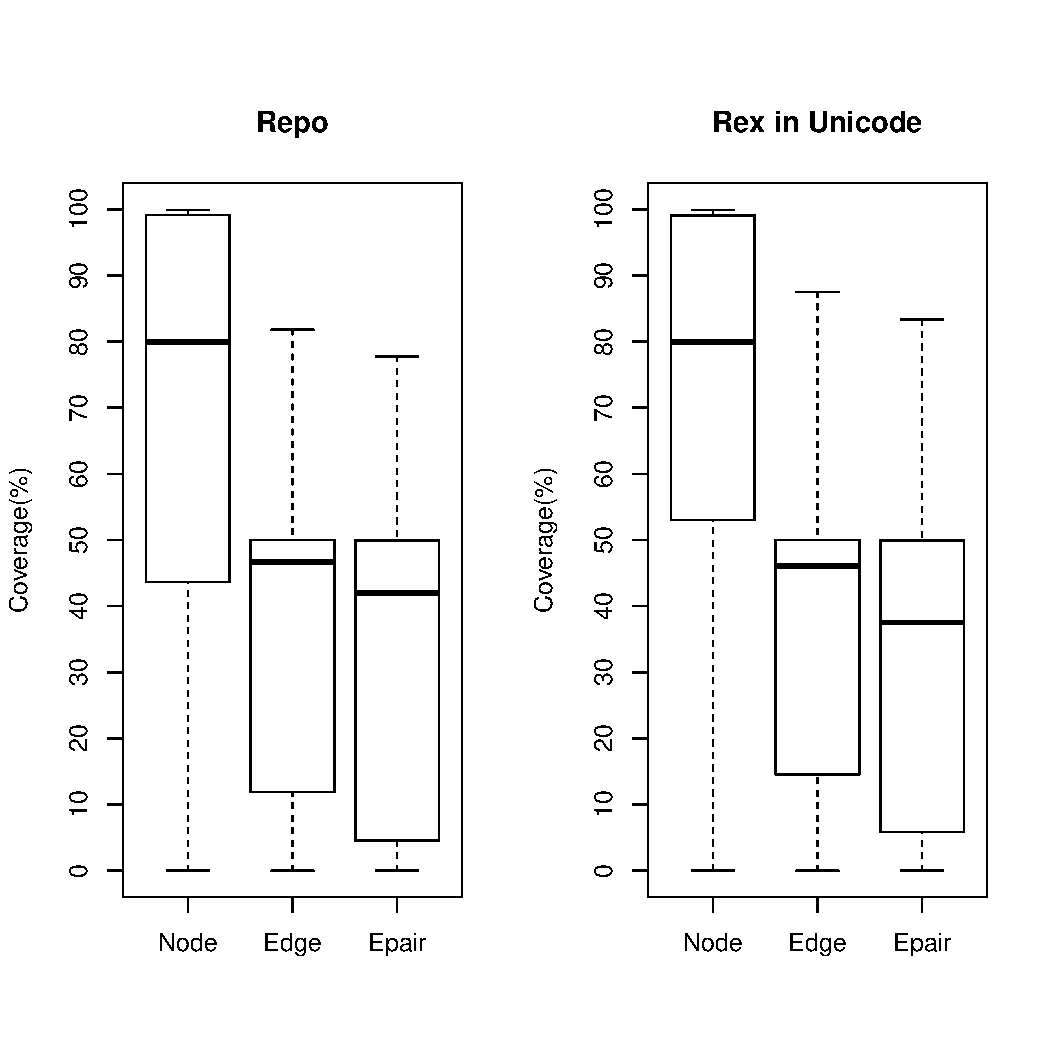
\includegraphics[width=0.5\textwidth]{figures/rexCovUnicodeS1}
	\vspace{-6pt}
	\caption{Node, edge, edge-pair coverage of 7,135 regular expressions with Rex-generated Unicode inputs of successful matchings from Rex and with the number of successful inputs in GitHub projects}
	\label{cov:unicode}    
	\vspace{-6pt}
\end{figure}
\fi
% Please add the following required packages to your document preamble:
% \usepackage{multirow}
%\begin{table}[t]
%\centering
%\caption{Averages of the testing coverage metrics in different dataset}
%\label{rex:compare}
%\begin{tabular}{l|l|l|l|ll}
%\hline
%\multirow{2}{*}{\begin{tabular}[c]{@{}l@{}}Coverages\\ (average)\end{tabular}} & Original & \multicolumn{2}{l|}{Rex ASCII} & \multicolumn{2}{l}{Rex Unicode}    \\ \cline{2-6} 
%                                                                               & Total    & All            & Same          & \multicolumn{1}{l|}{All}   & Same  \\ \hline
%Nodes(\%)                                                                      & 64.99    & 71.57          & 69.56         & \multicolumn{1}{l|}{71.57} & 69.56 \\
%Edges(\%)                                                                      & 31.72    & 36.59          & 34.40         & \multicolumn{1}{l|}{36.59} & 34.40 \\
%Edge pairs(\%)                                                                 & 23.85    & 29.37          & 26.25         & \multicolumn{1}{l|}{29.37} & 26.25 \\ \hline
%\end{tabular}
%\end{table}

\iffalse
\begin{table}[t]
\centering
\caption{Distribution of successful matchings and failed matchings for coverage calculation with different datasets}
\label{rex:succ}
\begin{small}
\begin{tabular}{p{2cm}
>{\raggedleft\arraybackslash}p{0.6cm}
>{\raggedleft\arraybackslash}p{0.6cm}
>{\raggedleft\arraybackslash}p{0.6cm}}
\hline
Dataset & total & succ & fail  \\  
\hline
GitHub& 15,096 & 10,155 & 4,941 \\  
Rex(ASCII)& 12,184 & 7,926 & 4,258 \\  
Rex(Unicode)& 12,181 & 7,924 & 4,257 \\
\hline
\end{tabular}
\end{small}
\end{table}

\begin{table}[tb]
\caption{Description of 7,924 regular expressions analyzed in Rex of Unicode encoding.}
\label{succ:unicode}
\begin{small}
\begin{tabular}{p{2cm}
>{\raggedleft\arraybackslash}p{0.6cm}
>{\raggedleft\arraybackslash}p{0.6cm}
>{\raggedleft\arraybackslash}p{0.6cm}
>{\raggedleft\arraybackslash}p{0.6cm}
>{\raggedleft\arraybackslash}p{0.6cm}
>{\raggedleft\arraybackslash}p{0.6cm}}
\hline
Attributes & mean & 25\% & 50\% & 75\% & 90\% & 99\%  \\  
\hline
Nodes& 220 & 13 & 31 & 162 & 618 & 970 \\  
Edges& 773 & 30 & 97 & 663 & 1,468 & 3,699 \\  
Edge pairs& 2,423 & 36 & 186 & 1,022 & 1,999 & 21,274 \\
Unique succ inputs& 34 & 1 & 1 & 2 & 8 & 208  \\   
Regular exp. len. & 29  & 12 & 15 & 31 & 71 & 160 \\
Input length avg. &  &  &  &  &  &  \\  
Input length dev. &  &  &  &  &  &  \\
\hline
\end{tabular}

\vspace{3pt}
All deviations are rounded to 2 decimal places. All input length averages are rounded to nearest integer.
\end{small}
\end{table}
\fi
%\subsection{Results}
%\adh{table references in this section are broken}
Figure~\ref{cov:ascii} shows the analysis results given the generated inputs in ASCII encoding, organized by each of five datasets. %\RepoOneT presents the coverage of the 10,155 regular expressions over $S$ in GitHub whose $S_{succ}>1$. 
\RepoTwoT and \RepoTwoS show the coverages over $S$ and $S_{succ}$ of 7,926 regular expressions using the developer-defined test suite in GitHub and their details are in Table~\ref{rex:data4}.
\RexSOne, \RexSFive, and \RexSTen show the coverages of 7,926 regular expressions based on the Rex-generates test inputs with sizes of 1x, 5x, and 10x of the user-defined test suite, respectively. Coverage details are shown in Table~\ref{rex:data1}.
%he data is found in Table~\ref{rex:data7}. \emph{Repo2T} and \emph{Repo2S} show the coverage over 7,886 regular expressions in ~\ref{sec:rq2}---which is same as the 7,886 in Rex---over $S$ and $S_{succ}$, with data in Table~\ref{rex:data4}. \emph{RexS1} shows the coverage over 7,886 regular expressions from Rex over $S_{succ}$, and Table~\ref{rex:data1} giving the details. \emph{RexS5} gives the coverage for 7,871 regular expressions from Rex whose input strings are five times as large as those in ~\ref{sec:rq2} with details in Table~\ref{rex:data2}. Finally, \emph{RexS10} is the coverage of 7,080 regular expressions whose input strings are ten times as large as those in~\ref{sec:rq2}, and the details are given in Table~\ref{rex:data3}.\adh{The strings are five/ten times larger or there are five/ten times as many strings?}





\iffalse
\begin{table}[tb]
%\centering
\caption{Description of 7,135 regular expression coverage for successful matchings in regular expressions in Rex and Unicode encoding. All numbers are rounded to two decimal places.}
\label{rex:data5}
\begin{small}
%\resizebox{0.5\textwidth}{!}{%
%\begin{tabular}{lllllllll}
\begin{tabular}{p{1cm}p{1cm}
>{\raggedleft\arraybackslash}p{0.6cm}
>{\raggedleft\arraybackslash}p{0.6cm}
>{\raggedleft\arraybackslash}p{0.6cm}
>{\raggedleft\arraybackslash}p{0.6cm}
>{\raggedleft\arraybackslash}p{0.6cm}
>{\raggedleft\arraybackslash}p{0.6cm}}
\hline
Coverage & Suite & mean & 25\% & 50\% & 75\% & 90\% & 99\%  \\
\hline
% for rex unicode coverages
NC (\%)& $S_{succ}$  & 73.88 & 53.02   & 80.00   & 99.12   & 99.85  & 99.90  \\  
EC (\%)& $S_{succ}$  & 34.64 & 14.53   & 46.11   & 49.97   & 50.00  & 68.57   \\
EPC (\%)& $S_{succ}$ & 30.15 & 5.86    & 37.50   & 49.96   & 50.00  & 61.98   \\
\hline
\end{tabular}
\end{small}
\end{table}

\begin{table}[tb]
%\centering
\caption{Description of 7,135 regular expression coverage for successful matchings in regular expressions in Github and Unicode encoding. All numbers are rounded to two decimal places.}
\label{rex:data6}
\begin{small}
%\resizebox{0.5\textwidth}{!}{%
%\begin{tabular}{lllllllll}
\begin{tabular}{p{1cm}p{1cm}
>{\raggedleft\arraybackslash}p{0.6cm}
>{\raggedleft\arraybackslash}p{0.6cm}
>{\raggedleft\arraybackslash}p{0.6cm}
>{\raggedleft\arraybackslash}p{0.6cm}
>{\raggedleft\arraybackslash}p{0.6cm}
>{\raggedleft\arraybackslash}p{0.6cm}}
\hline
Coverage & Suite & mean & 25\% & 50\% & 75\% & 90\% & 99\%  \\
% for github repo same regex as unicode coverages
NC (\%)& $S_{succ}$ & 70.74 & 43.71 & 80.00  & 99.13 & 99.85  & 99.90   \\
EC (\%)& $S_{succ}$ & 33.68 & 11.90 & 46.67  & 49.97   & 50.00  & 62.50   \\
EPC (\%)& $S_{succ}$& 29.68 & 4.52  & 42.11  & 49.97  & 50.00  & 58.52   \\
\hline
\end{tabular}
\end{small}
\end{table}


\begin{table}[tb]
%\centering
\caption{Description of 10,155 regular expression coverage for successful matchings in regular expressions in Github and Unicode encoding. All numbers are rounded to two decimal places. %\todo{I thought we were dropping the unicode results}}
\label{rex:data7}
\begin{small}
%\resizebox{0.5\textwidth}{!}{%
%\begin{tabular}{lllllllll}
\begin{tabular}{p{1cm}p{1cm}
>{\raggedleft\arraybackslash}p{0.6cm}
>{\raggedleft\arraybackslash}p{0.6cm}
>{\raggedleft\arraybackslash}p{0.6cm}
>{\raggedleft\arraybackslash}p{0.6cm}
>{\raggedleft\arraybackslash}p{0.6cm}
>{\raggedleft\arraybackslash}p{0.6cm}}
\hline
Coverage & Suite & mean & 25\% & 50\% & 75\% & 90\% & 99\%  \\
\hline
% for github repo all matchings coverages
NC (\%)& $S$ & 73.64 & 47.59 & 86.67  & 99.77 & 100.00  & 100.00   \\
EC (\%)& $S$ & 36.72 & 13.02 & 49.84  & 50.00   & 57.14  & 83.33   \\
EPC (\%)& $S$& 31.58 & 5.45  & 46.43  & 50.00  & 50.00  & 71.43   \\
\hline
% for github repo all successful matchings coverages
NC (\%)& $S_{succ}$ & 71.11 & 45.99 & 83.33  & 95.24 & 99.80  & 99.90   \\
EC (\%)& $S_{succ}$ & 34.48 & 12.13 & 48.53  & 50.00   & 50.00  & 62.50   \\
EPC (\%)& $S_{succ}$& 30.45 & 5.08  & 43.59  & 50.00  & 50.00  & 58.53   \\
\hline
\end{tabular}
%}
\end{small}
%
%\vspace{5pt}
%
%\vspace{-12pt}
\end{table}
\fi

\begin{table}[tb]
%\centering
%\caption{Description of 7,886 regular expression coverage for successful matchings in regular expressions in GitHub and ASCII encoding. All numbers are rounded to two decimal places.}
%\caption{Coverages of the 10,155 (\RepoOneS, \RepoOneT) regular expressions in GitHub whose $S_{succ}>1$ and coverages of the 7,926 (\RepoTwoS, \RepoTwoT) regular expressions in GitHub whose $S_{succ}>1$ and which are used in Rex.}
\caption{Coverage values of the 7,926 regular expressions in GitHub for \RepoTwoS and \RepoTwoT in Figure~\ref{cov:ascii}.}
\label{rex:data4}
\vspace{-6pt}
\begin{small}
%\resizebox{0.5\textwidth}{!}{%
%\begin{tabular}{lllllllll}
\begin{tabular}{p{1cm}p{1cm}
>{\raggedleft\arraybackslash}p{0.6cm}
>{\raggedleft\arraybackslash}p{0.6cm}
>{\raggedleft\arraybackslash}p{0.6cm}
>{\raggedleft\arraybackslash}p{0.6cm}
>{\raggedleft\arraybackslash}p{0.6cm}
>{\raggedleft\arraybackslash}p{0.6cm}}
\hline
Coverage & Expr & mean & 25\% & 50\% & 75\% & 90\% & 99\%  \\
%\hline
%% for github repo same regex as ascii coverages 7886
%NC (\%)& \RepoTwoS & 70.44 & 43.75 & 80.00  & 97.78 & 99.84  & 99.90   \\
%EC (\%)& \RepoTwoS & 33.82 & 11.99 & 46.15   & 49.97   & 50.00  & 66.67   \\
%EPC (\%)& \RepoTwoS & 29.45 & 4.79  & 37.50   & 49.97  & 50.00  & 60.00   \\
%\hline
%\hline
%% for github repo same regex as ascii coverages 7886
%NC (\%)& \RepoTwoT & 73.29 & 46.15 & 85.71  & 99.83 & 100.00  & 100.00   \\
%EC (\%)& \RepoTwoT & 36.39 & 12.32 & 48.72   & 49.97   & 60.00  & 85.71   \\
%EPC (\%)& \RepoTwoT & 30.75 & 5.13  & 40.00   & 49.97  & 50.00  & 75.00   \\
%\hline
%\hline
%NC (\%)& \RepoOneT   & 59.05 & 24.62   & 63.64  & 95.65   & 100.00 & 100.00   \\
%EC (\%)& \RepoOneT   & 28.74 & 6.67   & 23.90   & 49.97   & 53.80  & 80.00  \\  
%EPC (\%)&\RepoOneT &23.77    & 2.47    & 12.50  & 49.96  & 50.00 & 66.67 \\
%\hline
\hline
% for github repo same regex as ascii coverages 7926 succ
NC (\%)& \RepoTwoS & 70.41 & 43.75 & 80.00  & 97.67 & 99.84  & 99.90   \\
EC (\%)& \RepoTwoS & 33.79 & 12.01 & 45.91  & 49.97  & 50.00  & 66.67   \\
EPC (\%)& \RepoTwoS & 29.39 & 4.83  & 37.50   & 49.97  & 50.00  & 60.00   \\
\hline
\hline
% for github repo same regex as ascii coverages 7926 total
NC (\%)& \RepoTwoT & 73.27 & 46.15 & 85.71  & 99.83 & 100.00  & 100.00   \\
EC (\%)& \RepoTwoT & 36.35 & 12.36 & 48.39  & 49.97   & 60.00  & 85.71   \\
EPC (\%)& \RepoTwoT & 30.68 & 5.13 & 40.00  & 49.97  & 50.00  & 74.67   \\
%\hline
%\hline
%% for github repo same regex as ascii coverages 10155 succ
%NC (\%)& \RepoOneS & 71.11 & 45.99  & 83.33  & 95.24   & 99.80 & 99.90   \\
%EC (\%)& \RepoOneS & 34.48 & 12.13  & 48.53  & 50.00  & 50.00  & 62.50  \\  
%EPC (\%)&\RepoOneS & 30.45 & 5.08   & 43.59  & 50.00  & 50.00  & 58.33 \\
\hline
% for github repo same regex as ascii coverages 10155 total
%NC (\%)& \RepoOneT & 73.64 & 47.59  & 86.67  & 99.77   & 100.00 & 100.00   \\
%EC (\%)& \RepoOneT & 36.72 & 13.02   & 49.84  & 50.00  & 57.14  & 83.33  \\  
%EPC (\%)&\RepoOneT & 31.58 & 5.45    & 46.43  & 50.00  & 50.00  & 71.43 \\
%\hline

\end{tabular}
\end{small}
\vspace{-3pt}
\end{table}




\begin{table}[tb]
%\centering
%\caption{Coverage of the 7,886 (\RexSOne); 7,871 (\RexSFive); 7,080 (\RexSTen) regular expressions using Rex. All numbers are rounded to two decimal places. \todo{how is it possible that \RexSTen coverage goes down? Is this because the regular expressions we dropped have finite languages? Check on it.}}
%\caption{Coverage of the 7,926 regular expressions using Rex for \RexSOne, \RexSFive, and \RexSTen. All numbers are rounded to two decimal places.}
\caption{Coverage values of the 7,926 regular expressions using Rex for \RexSOne, \RexSFive, and \RexSTen in Figure~\ref{cov:ascii}.}
\label{rex:data1}
\vspace{-6pt}
\begin{small}
%\resizebox{0.5\textwidth}{!}{%
%\begin{tabular}{lllllllll}
\begin{tabular}{p{1cm}p{1cm}
>{\raggedleft\arraybackslash}p{0.6cm}
>{\raggedleft\arraybackslash}p{0.6cm}
>{\raggedleft\arraybackslash}p{0.6cm}
>{\raggedleft\arraybackslash}p{0.6cm}
>{\raggedleft\arraybackslash}p{0.6cm}
>{\raggedleft\arraybackslash}p{0.6cm}}
\hline
Coverage & Expr & mean & 25\% & 50\% & 75\% & 90\% & 99\%  \\
%\hline
%% for rex ascii coverages
%NC (\%)& \RexSOne & 70.19 & 43.75 & 80.00  & 97.62 & 99.84  & 99.90   \\
%EC (\%)& \RexSOne & 33.95 & 11.93   & 45.63   & 49.97   & 50.00  & 71.43   \\
%EPC (\%)& \RexSOne & 29.78 & 4.55    & 36.52   & 49.96  & 50.00  & 66.67   \\
%\hline
%\hline
%% for rex ascii coverages scale 5
%NC (\%)&\RexSFive & 72.08 & 46.15 & 83.33  & 97.78 & 99.84  & 99.90   \\
%EC (\%)& \RexSFive & 36.59 & 13.05   & 49.83   & 50.00  & 54.55  & 80.00   \\
%EPC (\%)& \RexSFive & 33.22 & 6.78    & 49.63   & 50.00  & 56.67  & 75.00   \\
%\hline
%\hline
%% for rex ascii coverages scale 10
%NC (\%)& \RexSTen & 70.56 & 42.32 & 80.00  & 99.17 & 99.85  & 99.90   \\
%EC (\%)& \RexSTen & 35.58 & 12.20  & 48.48   & 49.97  & 57.14  & 80.00   \\
%EPC (\%)& \RexSTen & 32.22 & 6.12    & 44.77   & 49.97  & 58.33  & 75.00   \\
%\hline
\hline
% for rex ascii coverages 7926
NC (\%)& \RexSOne & 69.29 & 41.67 & 78.33  & 97.44 & 99.84  & 99.90   \\
EC (\%)& \RexSOne & 33.57 & 11.62   & 45.00   & 49.97   & 50.00  & 71.43   \\
EPC (\%)& \RexSOne & 29.50 & 4.33    & 35.00   & 49.96  & 50.00  & 66.67   \\
\hline
\hline
% for rex ascii coverages scale 5 7926
NC (\%)&\RexSFive & 71.69 & 46.15 & 83.33  & 97.67 & 99.84  & 99.90   \\
EC (\%)& \RexSFive & 36.42 & 12.77   & 49.81   & 50.00  & 54.55  & 80.00   \\
EPC (\%)& \RexSFive & 33.04 & 6.63   & 49.54   & 50.00  & 56.67  & 75.00   \\
\hline
\hline
% for rex ascii coverages scale 10 7926
NC (\%)& \RexSTen & 72.01 & 46.15 & 83.33  & 97.73 & 99.84  & 99.90   \\
EC (\%)& \RexSTen & 36.87 & 13.39 & 49.85  & 50.00  & 55.89  & 80.00   \\
EPC (\%)& \RexSTen & 33.77 & 6.90 & 49.77  & 50.00  & 58.33  & 75.00   \\
\hline
\end{tabular}
\end{small}
\vspace{-6pt}
\end{table}


\begin{table}[tb]
\caption{Differences in coverage based on datasets in Figure~\ref{cov:ascii}. Hypothesis tests used paired Wilcoxon signed-rank test. Bold text identifies when one of the datasets had significantly higher coverage for all three metrics. If there was a conflict between the metrics (e.g., Set1 $>$ Set2 for NC, and Set1 $<$ Set2 for EPC), there was no winner}
\label{rq2hypothesistests}
\vspace{-6pt}
\begin{tabular}{l l | r r r}
\hline
& & \multicolumn{3}{c}{$H_0: {Set1} \,{\buildrel d \over =}\, {Set2}$}\\
Set1 & Set2 & NC & EC & EPC \\ \hline 
\textbf{\RepoTwoS} & \RexSOne & p $<$ 0.0001 & p $<$ 0.0001 & p $<$ 0.0001\\ %$< 2.2 \times 10^{-16}$ & p $< 2.2 \times 10^{-16}$ & p = $6.12 \times 10^{-8}$ \\
\RepoTwoS & \textbf{\RexSFive} & p $<$ 0.0001 & p $<$ 0.0001 & p $<$ 0.0001\\ 
\RepoTwoS & \textbf{\RexSTen} & p $<$ 0.0001 & p $<$ 0.0001 & p $<$ 0.0001\\ 
\hline \hline
\textbf{\RepoTwoT} & {\RexSOne} & p $<$ 0.0001 & p $<$ 0.0001 & p $<$ 0.0001\\ 
\RepoTwoT & {\RexSFive} & p $<$ 0.0001 & p $=$ 0.0004 & p $<$ 0.0001\\ 
\RepoTwoT & {\RexSTen} & p $<$ 0.0001 & p $=$ 0.4147 & p $<$ 0.0001\\ 
\hline \hline
\textbf{\RepoTwoT} & {\RepoTwoS} & p $<$ 0.0001 &  p $<$ 0.0001  & p $<$ 0.0001\\ 
\hline
\end{tabular}
\vspace{-12pt}
\end{table}




Table~\ref{rq2hypothesistests} illustrates the differences in coverage between the repository (\RepoTwoS and \RepoTwoT) and Rex (\RexSOne, \RexSFive, and \RexSTen). Using a paired Wilcoxon signed-rank test, we find that for all three coverage metrics, \RepoTwoS significantly outperforms \RexSOne  with $\alpha = 0.0001$. However, as test suite size is strongly correlated with coverage~\cite{coveragetestsuitecorrelation}, as soon as the Rex test set is amplified to 5x and 10x the size, the coverage of Rex outperforms the repository. 
When considering all test inputs from the repository and not just the successful ones, with test inputs sets of the same size, \RepoTwoT outperforms \RexSOne. However,  this comparison is unfair since Rex does not generate non-matching strings. That said, as soon as the Rex dataset is amplified as in \RexSFive and \RexSTen, there is no clear winner compared to all test inputs from the repository. 
While it may appear that Rex can do as well as the repository, the reality is that the error node will never be covered by Rex, a fact which is not apparent by looking at the numbers alone.  
%From Figure~\ref{cov:ascii} we found that differences between \emph{Repo2S} and \emph{RexS1} are not significant, suggesting that for the same number of input strings Rex-generated inputs are not very helpful. This is because that for 5,361 of the 7,886 regular expressions their $S_{succ}$ contain single input string. With a single path from $N_0$ to $N_m$, the coverage could not be improved much. The benefits of automatically generated inputs are shown in \emph{RexS5} and \emph{RexS10}. There is a significant increase for edge-pair coverage. The medians of both the edge and edge-pair coverage have moved closer to 50\%. It implies that the regular expression coverage can be improved with more Rex-generated input strings. However, the medians of both the edge and edge-pair coverage have not exceeded 50\% meaning that there is a ceiling for {\em EC} and {\em EPC} over the test suite $S_{succ}$ and thus the coverage improvements gained from Rex is limited when the medians of edge and edge-pair coverage are close to 50\%. To achieve additional coverage improvements, we can consider more inputs in $S_{fail}$.




%\paragraph{Summary:}
\textbf{Summary:}
Rex can handle approximately 78.1\% of the regular expressions from our dataset. % collected for RQ1. 
Considering only the matching test inputs and test sets of the same size, Rex does not achieve coverage as high as the developer-written tests. However, the coverage numbers are extremely close. This indicates that tools such as Rex can be used to write test inputs with similar coverage to the developer tests, but will always miss $N_e$ and all edges incident to it. 
%Rex does help increase the testing coverage of regular expressions to a certain degree. However, the benefit is restricted to \todo{node coverage?} and the tool is only helpful for \todo{scope} of regular expression.s. \todo{check this after the hypothesis tests}

